% Autor: Leonhard Segger, Alexander Neuwirth
% Datum: 2017-10-30
\documentclass[
	% Papierformat
	a4paper,
	% Schriftgröße (beliebige Größen mit „fontsize=Xpt“)
	12pt,
	% Schreibt die Papiergröße korrekt ins Ausgabedokument
	pagesize,
	% Sprache für z.B. Babel
	ngerman
]{scrartcl}

% Achtung: Die Reihenfolge der Pakete kann (leider) wichtig sein!
% Insbesondere sollten (so wie hier) babel, fontenc und inputenc (in dieser
% Reihenfolge) als Erstes und hyperref und cleveref (Reihenfolge auch hier
% beachten) als Letztes geladen werden!

\usepackage{tikz}
\usetikzlibrary{calc,patterns,angles,quotes} % loads some tikz extensions\usepackage{tikz}
\usetikzlibrary{babel}

% Silbentrennung etc.; Sprache wird durch Option bei \documentclass festgelegt
\usepackage{babel}
% Verwendung der Zeichentabelle T1 (Sonderzeichen etc.)
\usepackage[T1]{fontenc}
% Legt die Zeichenkodierung der Eingabedatei fest, z.B. UTF-8
\usepackage[utf8]{inputenc}
% Schriftart
\usepackage{lmodern}
% Zusätzliche Sonderzeichen
\usepackage{textcomp}

% Mathepaket (intlimits: Grenzen über/unter Integralzeichen)
\usepackage[intlimits]{amsmath}
% Ermöglicht die Nutzung von \SI{Zahl}{Einheit} u.a.
\usepackage{amssymb}
% mehr symbole plox
\usepackage{siunitx}
% Zum flexiblen Einbinden von Grafiken (\includegraphics)
\usepackage{graphicx}
% Abbildungen im Fließtext
\usepackage{wrapfig}
% Abbildungen nebeneinander (subfigure, subtable)
\usepackage{subcaption}
% Funktionen für Anführungszeichen
\usepackage{csquotes}
\MakeOuterQuote{"}
% Zitieren, Bibliografie
\usepackage[sorting=none]{biblatex}


% Zur Darstellung von Webadressen
\usepackage{url}
%chemische Formeln
\usepackage[version=4]{mhchem}
% siunitx: Deutsche Ausgabe, Messfehler getrennt mit ± ausgeben
\usepackage{floatrow}
\floatsetup[table]{capposition=top}
\usepackage{float}
% Verlinkt Textstellen im PDF-Dokument
\usepackage[unicode]{hyperref}
% "Schlaue" Referenzen (nach hyperref laden!)
\usepackage{cleveref}
\sisetup{
	locale=DE,
	separate-uncertainty
}
\bibliography{References}

\begin{document}

	\begin{titlepage}
		\centering
		{\scshape\LARGE Versuchsbericht zu \par}
		\vspace{1cm}
		{\scshape\huge Optische Fouriertransformation \par}
		\vspace{2.5cm}
		{\LARGE Gruppe BA-C-04 \par}
		\vspace{0.5cm}

		{\large Alexander Neuwirth (E-Mail: a\_neuw01@wwu.de) \par}
		{\large Leonhard Segger (E-Mail: l\_segg03@uni-muenster.de) \par}
		\vfill

		durchgeführt am 17.06.2019\par
		betreut von\par
		{\large Florian Schepers}

		\vfill

		{\large \today\par}
	\end{titlepage}
	\tableofcontents
	\newpage


	\section{Kurzfassung}
	% Hypothese	und deren Ergebnis, wenn Hypothese ist, dass nur Theorie erfüllt, sagen: Erwartung: Theorie aus einführung (mit reflink) erfüllt
	% Ergebnisse, auch Zahlen, mindestens wenn's halbwegs Sinn ergibt
	% Was wurde gemacht
	% manche leute wollen Passiv oder "man", manche nicht

  \section{Theorie}
	% wdh. Texte
	% wdh. Besprechung


	\section{Grundaufbau}
	Es wird ein Helium-Neon-Laser auf einer \SI{4}{m} langen optischen Bank montiert.
	Am anderen Ende der Bank wird ein halbtransparenter Schirm aufgestellt, auf den von Hinten eine Digitalkamera gerichtet und fokussiert wird. %TODO "halbtransparent"?
	Der Laser wird mithilfe einer Lochblende parallel zur optischen Bank ausgerichtet.
	Wenn im Folgenden Linsen eingesetzt werden, wird mithilfe einer Markierung auf einem Schirm sichergestellt, dass der Laserstrahl nach Durchgang durch die Linse noch immer im Mittel parallel zur optischen Bank verläuft, der Laser also mittig durch die Linse läuft. %TODO im Mittel, weil ja nicht jeder Teilstrahl parallel ist. theoretisch auch im vorigen Satz
	Es wird die Länge in Pixeln eines Abstandes von \SI{10}{cm} anhand eines Lineals auf dem Schirm anhand der Digitalaufnahme gemessen, um den Umrechnungsfaktor von Pixeln in Abstand auf dem Schirm zu bestimmen.
	%TODO kp, ob du den Umrechnungsfaktor irgendwo hinpacken willst. und wo.
	Im Folgenden wird die Belichtungszeit der Kamera für jede Aufnahme individuell eingestellt, um eine optimale Abzählung der Peaks zu ermöglichen.
	Hierfür wird auch eine Überbelichtung in Kauf genommen.
	Dies verhindert einen Vergleich der Intensitäten zwischen einzelnen Aufnahmen, aber ein solcher ist auch nicht notwendig.

	\begin{figure}[H]
			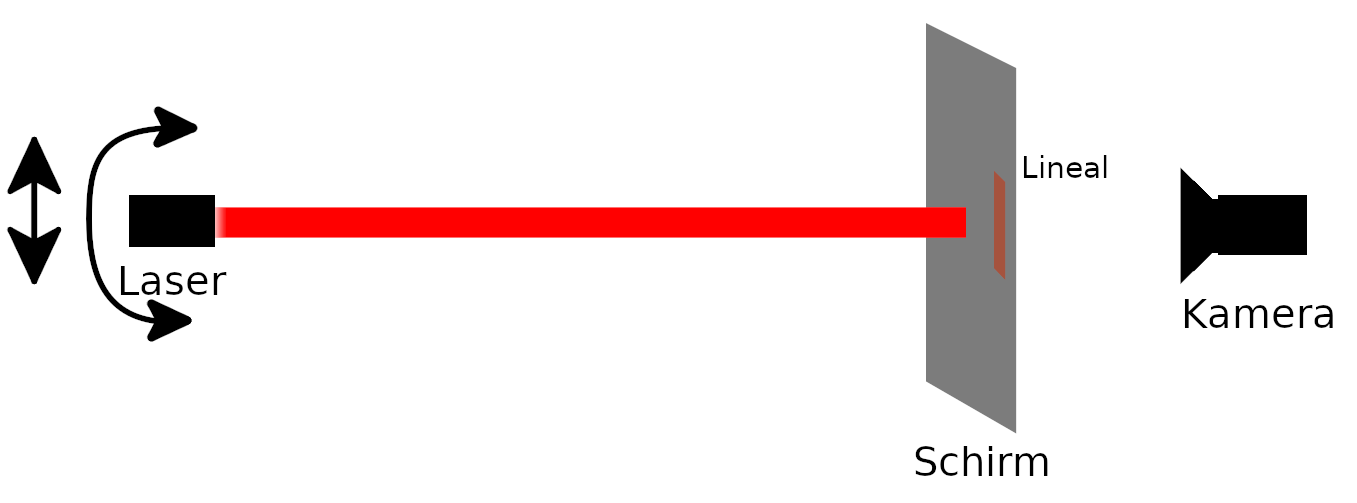
\includegraphics[width=1\linewidth]{img/grundaufbau}
			\caption{
				Der Grundaufbau. Der Laser wird parallel zur optischen Bank ausgerichtet.
			}
			\label{fig_grundaufbau}
	\end{figure}

	\section{Ergebnisse und Diskussion}
	%TODO ist das fine, dass ich das alles * gemacht habe?

	\subsection{Unsicherheiten}
	%TODO Unsicherheiten


	\subsection{Übergang von Nah- zu Fernfeld}

	\subsubsection*{Methode}
	In den Strahlengang werden zwei Linsen mit $f_1=\SI{50}{mm}$ und $f_2=\SI{100}{mm}$ in einem Abstand von \SI{170}{mm} gebracht, um den Strahl zu kollimieren.
  Dann wird ein Gitter (später Gitter Nr.2) in den Strahl gebracht und in verschiedenen Abständen das Bild auf dem Schirm aufgenommen.

		\begin{figure}[H] %TODO Abstand d kann ich in alles ändern.
			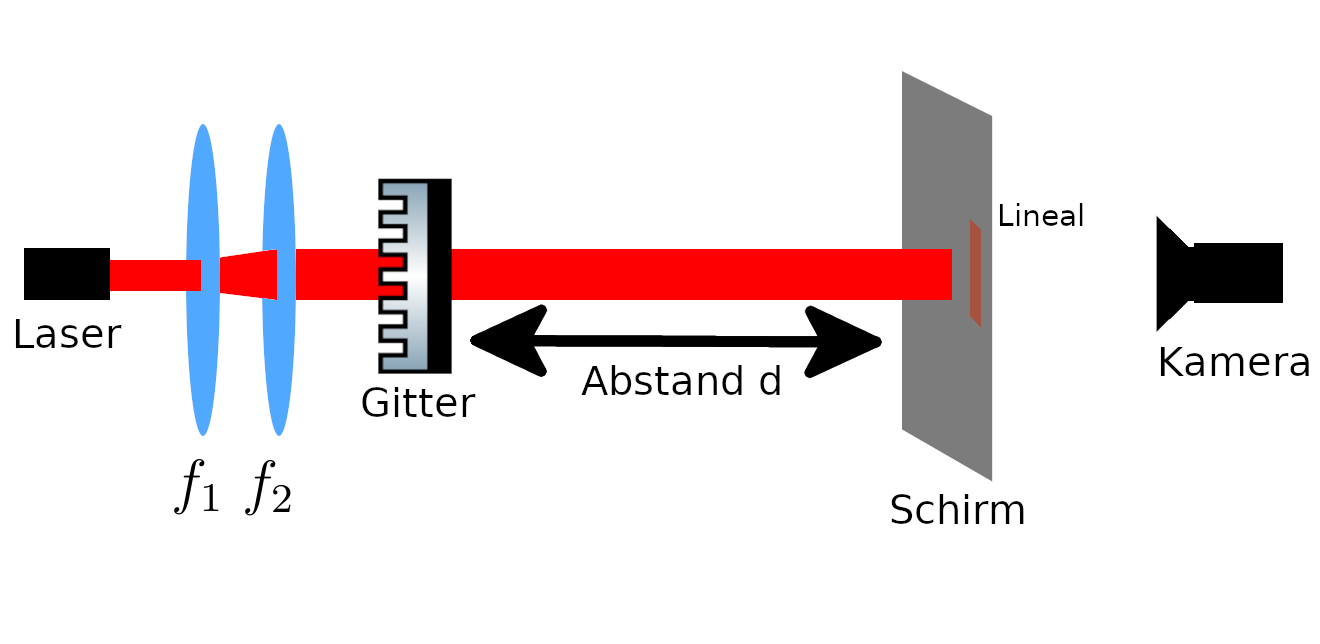
\includegraphics[width=1\linewidth]{img/nahfern}
					\caption{
						Aufbau zum Vergleich von Nah- und Fernfeld. Der Abstand zwischen den Kollimierungslinsen beträgt \SI{170}{mm}
					}
					\label{fig_nahfern}
			\end{figure}


	\subsubsection*{Beobachtung und Datenanalyse}
	% Allgemeine Beobachtungen
	% Einflüsse von veränderten Parametern auf Messung

	\subsubsection*{Diskussion}
	% Bezug/Nutzen oder sonst was
	% auch hier die Hypothese wiederholen
	% keine Messwerte hier, nach manchen Menschen, zumindest "direkt" erstellte Diagramme net hier, auch wenn Lesbarkeit-bla


	\subsection{Bestimmung von Gitterkonstanten}

	\subsubsection*{Methode}

	Es wird derselbe Aufbau wie zuvor verwendet (vgl. \cref{fig_nahfern}).
	Dann wird mit einem Abstand von \SI{2,715}{m} zwischen Gitter und Schirm das Beugungsbild für fünf verschiedene Gitter aufgenommen.

	\subsubsection*{Beobachtung und Datenanalyse}
	% Allgemeine Beobachtungen
	% Einflüsse von veränderten Parametern auf Messung

	\subsubsection*{Diskussion}
	% Bezug/Nutzen oder sonst was
	% auch hier die Hypothese wiederholen
	% keine Messwerte hier, nach manchen Menschen, zumindest "direkt" erstellte Diagramme net hier, auch wenn Lesbarkeit-bla


	\subsection{Fouriertransformation mit einer Linse}
		%TODO hier ist halt weird, dass das nicht so wirklich Fourier ist, aber es ist wohl das aus der Unendlichkeit holen gemeint (Das Fernfeld ist halt instant da.)


	\subsubsection*{Methode}

		Der vorherige Versuchsteil wird mit dem Unterschied, dass sich nun eine Linse zwischen Schirm und Gitter befindet, widerholt.
		Die Linse wird so eingebaut, dass sich Schirm und Gitter in je einer der Fokusebenen befinden.

	\begin{figure}[H]
			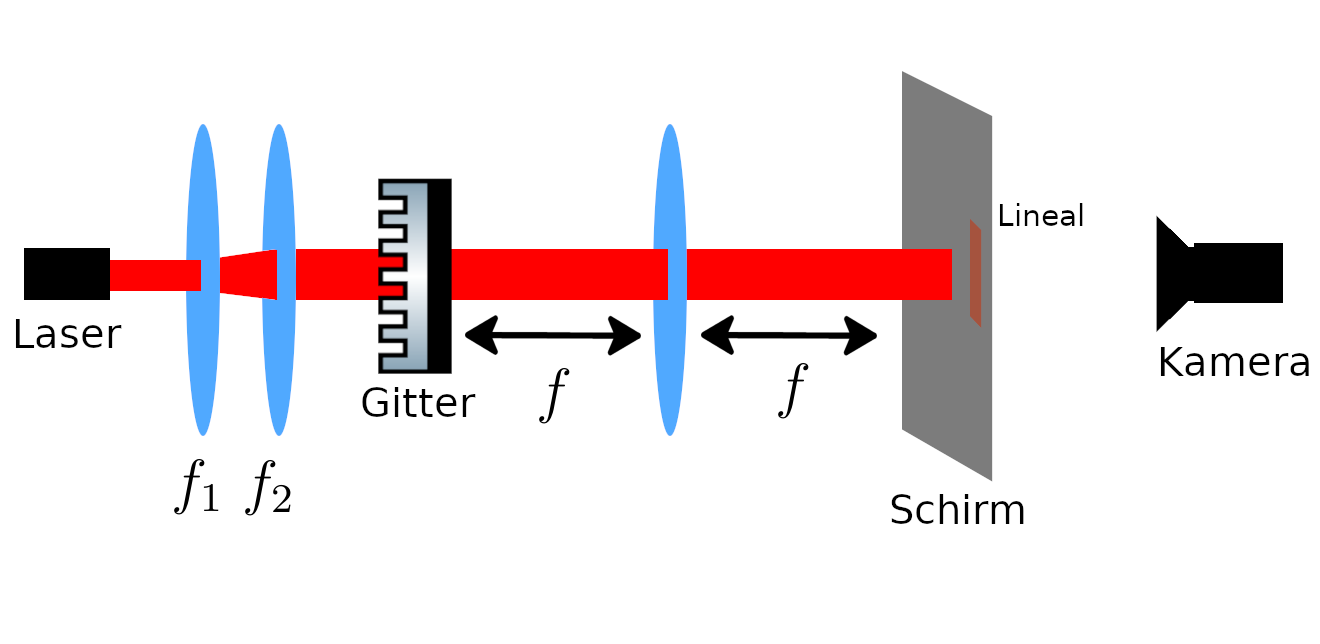
\includegraphics[width=1\linewidth]{img/gitterlinse}
			\caption{
				Aufbau zur Bestimmung der Abstände der Beugungsordnungen. Die zusätzlich eingebaute Linse steht im Abstand $f=\SI{500}{mm}$ zu Gitter und Schirm.
			}
			\label{fig_gitterlinse}
	\end{figure}

	\subsubsection*{Beobachtung und Datenanalyse}
	% Allgemeine Beobachtungen
	% Einflüsse von veränderten Parametern auf Messung
	%TODO Überstrahlung nahe 0. Ordnung verhindert Zählen -> Extrapolation der Ordnung aus Abstand
	%TODO bei g1 nichts zu erkennen -> Alternativversuche -> immer noch nicht.

	\subsubsection*{Diskussion}
	% Bezug/Nutzen oder sonst was
	% auch hier die Hypothese wiederholen
	% keine Messwerte hier, nach manchen Menschen, zumindest "direkt" erstellte Diagramme net hier, auch wenn Lesbarkeit-bla
%TODO man verlässt sich halt nicht auf Fernfeld, sondern bringt das Bild in die Endlichkeit.

	\subsection{Fourierfilterung}

	\subsubsection*{Methode}

		Der Strahl wird mit einem Linsenpaar auf einen Durchmesser von etwa \SI{50}{mm} aufgeweitet und kollimiert.
		Es wird ein 4f-Aufbau zur Fourierfilterung verwendet.
		Dieser ist in \cref{fig_4f} dargestellt.
		Dann werden mehrere Messungen mit unterschiedlichen Objekten und Filtern durchgeführt.

	\begin{figure}[H]
			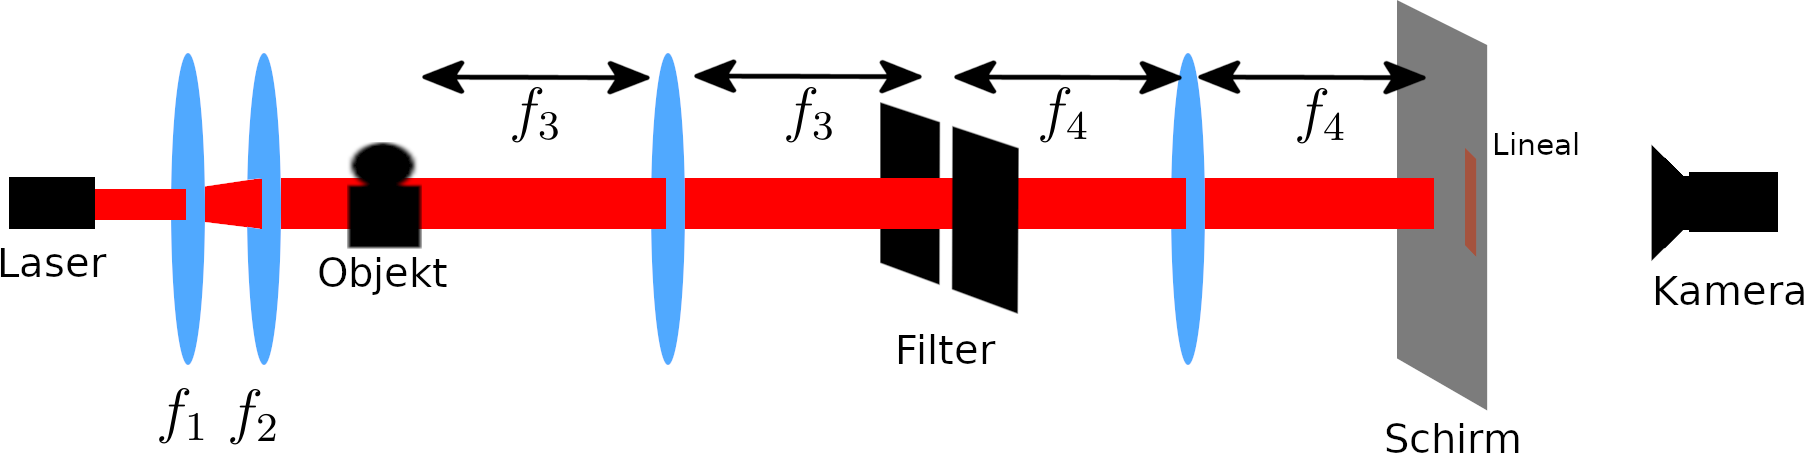
\includegraphics[width=1\linewidth]{img/4f}
			\caption{
				4f-Aufbau zur Fourierfilterung. $f_1= \SI{5}{mm}$, $f_2 = f_3 = f_4 = \SI{500}{mm}$. Es werden verschiedene Objekte und Filter verwendet.
			}
			\label{fig_4f}
	\end{figure}

		Zunächst wird der Schriftzug \enquote{Fourier} überlagert mit einem senkrechten Gitter als Objekt verwendet.
		Durch einen Tiefpassfilter wird dieser aus dem Bild entfernt.
		Der Tiefpassfilter wird durch einen schmalen horizontalen Spalt realisiert.

		Dann wird ein Bruch als Objekt verwendet, bei dem der Nenner mit einem Gitter überlagert ist.
		Um den Zähler aus dem Bruch zu entfernen, wird ein eindimensionaler Hochpassfilter in Form einer Nadel verwendet.
		%TODO Hier haben wir, denke ich, verkackt. Wir haben den Nenner entfernt.

		Nun wird ein Quadratgitter und ein Spalt als eindimensionaler Tiefpassfilter verwendet.
		Der Spalt wird im Winkel von \SI{0}{\degree}, \SI{45}{\degree} und \SI{90}{\degree} eingesetzt.

		Es wird als Objekt eine Schraube und als Filter ein Hochpassfilter in Form eines Kreises auf einer durchsichtigen Folie verwendet.

		Zuletzt wird, um die Dunkelfeldmethode zu verwenden, wie zuvor ein Hochpassfilter eingesetzt.
		Als Objekt werden die aufsteigenden Luftströme über einer Kerzenflamme verwendet.
		Damit diese besser sichtbar werden, werden Luftverwirbelungen per Hand eingebracht.

	\subsubsection*{Beobachtung und Datenanalyse}
	% Allgemeine Beobachtungen
	% Einflüsse von veränderten Parametern auf Messung

	\subsubsection*{Diskussion}
	% Bezug/Nutzen oder sonst was
	% auch hier die Hypothese wiederholen
	% keine Messwerte hier, nach manchen Menschen, zumindest "direkt" erstellte Diagramme net hier, auch wenn Lesbarkeit-bla
%TODO fourierschriftzug: Buchstabenfrequenz kleiner als gitter. Je mehr wegefiltert, desto unschärfer der Schriftzug.

	\section{Schlussfolgerung}
	% Rückgriff auf Hypothese und drittes Nennen dieser

	% Quellen zitieren, Websiten mit Zugriffsdatum
	% Verweise auf das Laborbuch (sind erlaubt)
	% Tabelle + Bilder mit Beschriftung
	\printbibliography
\end{document}


%TODO Einheiten bisschen anpassen, also alle Brennweiten in Millimeter und alle Abstände gleichmäßig.
